% Part: sets-functions-relations
% Chapter: arithmetization
% Section:reals

\documentclass[../../../include/open-logic-section]{subfiles}

\begin{document}

\olfileid{sfr}{arith}{real}
\olsection{The Real Line}

The next step is to show how to construct the reals from the
rationals. Before that, we need to understand what is
\emph{distinctive} about the reals. 

The reals behave very much like the rationals. (Technically, both are
examples of \emph{ordered fields}; for the definition of this, see
\olref[check]{orderedfield}.) Now, if you worked through the exercises
to \olref[sfr][siz][]{chap}, you will know that there are strictly
more reals than rationals, i.e., that $\cardless{\Rat}{\Real}$. This
was first proved by Cantor. But it's been known for about two and a
half millennia that there are irrational numbers, i.e., reals which
are not rational. Indeed:
%\footnote{Now: ``$\sqrt{2}$'' equally refers to both the positive and the negative roots; but in the next few pages, I'll forget about this, and consider only the positive root.}
\begin{thm}\ollabel{root2irrational}
$\sqrt{2}$ is not rational, i.e., $\sqrt{2} \notin \Rat$
\end{thm}

\begin{proof}
Suppose, for reductio, that $\sqrt{2}$ is rational. So $\sqrt{2} =
\nicefrac{m}{n}$ for some natural numbers $m$ and $n$. Indeed, we can
choose $m$ and $n$ so that the fraction cannot be reduced any further.
Re-organising, $m^{2} = 2n^{2}$. From here, we can complete the proof
in two ways:

\emph{First, geometrically} (following Tennenbaum).\footnote{This
proof is reported by \cite{Conway2006}.} Consider these squares:
\begin{center}	
	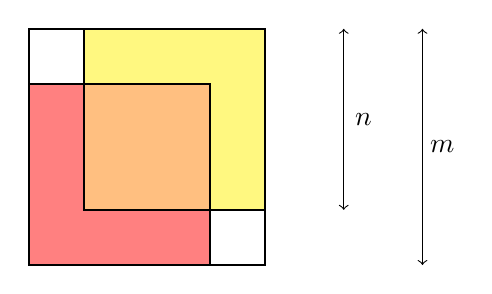
\begin{tikzpicture}
		\draw[thick] (0,0) rectangle (3,3);
		\draw[thick, fill=red!50] (0,0) rectangle (2.3,2.3);
		\draw[thick, fill=yellow!50] (0.7,0.7) rectangle (3, 3);
		\draw[thick, fill=orange!50] (0.7,0.7) rectangle (2.3, 2.3);
		\draw[<->] (4, 0.7)--(4, 3);
		\node at (4.25, 1.85) (n) {$n$};
		\draw[<->] (5, 0)--(5, 3);
		\node at (5.25, 1.5) (m) {$m$};
	\end{tikzpicture}
\end{center}
Since $m^2 = 2n^2$, the region where the two squares of side $n$
overlap has the same area as the region which neither of the two
squares cover; i.e., the area of the orange square equals the sum of
the area of the two unshaded squares. So where the orange square has
side $p$, and each unshaded square has side $q$, $p^2 = 2q^2$. But now
$\sqrt{2} = \nicefrac{p}{q}$, with $p < m$ and $q < n$ and $p, q \in
\Nat$. This contradicts the fact that $m$ and $n$ were chosen to be as
small as possible.
		
\emph{Second, formally.} Since $m^{2} = 2n^{2}$, it follows that $m$
is even. (It is easy to show that, if $x$ is odd, then $x^2$ is odd.)
So $m = 2r$, for some $r \in \Nat$. Rearranging, $2r^2 = n^2$, 
		%				\begin{align*}
		%					(2q)^{2} &= 2n^{2}\\
		%					4q^{2} &= 2n^{2}\\
		%					2q^{2} &= n^{2}
		%				\end{align*}
so $n$ is also even. So both $m$ and $n$ are even, and hence the
fraction $\nicefrac{m}{n}$ \emph{can} be reduced further.
Contradiction!
\end{proof}

In passing, this diagrammatic proof allows us to revisit the material from \olref[his][set][mythology]{sec}. Tennenbaum (1927--2006) was a thoroughly modern mathematician; but the proof is undeniably lovely, completely rigorous, and appeals to geometric intuition!

In any case: the reals are ``more expansive'' than the rationals. In some sense, there are ``gaps'' in the rationals, and these are filled by the reals. Weierstrass realised that this describes a single property of the real numbers, which distinguishes them from the rationals, namely the Completeness Property: \emph{Every non-empty set of real numbers with an upper bound has a least upper bound.} 

It is easy to see that the rationals do not have the Completeness Property. For example, consider the set of rationals less than $\sqrt{2}$, i.e.:
\[
	\Setabs{p \in \Rat}{p^2 < 2 \text{ or }p < 0}
\]
This has an upper bound in the rationals; its !!{elements} are all  smaller than $3$, for example. But what is its least upper bound? We want to say `$\sqrt{2}$'; but we have just seen that $\sqrt{2}$ is \emph{not} rational. And there is no \emph{least} rational number greater than $\sqrt{2}$. So the set has an upper bound but no least upper bound. Hence the rationals lack the Completeness Property.

By contrast, the continuum ``morally ought'' to have the Completeness Property. We do not just want $\sqrt{2}$ to be a real number; we want to fill all the ``gaps'' in the rational line. Indeed, we want the continuum itself to have no ``gaps'' in it. That is just what we will get via Completeness.

\end{document}